\chapter{Landasan Teori}
\label{chap:landasan_teori}

Dari topik yang ada, akan dipilah-pilah menjadi beberapa komponen penyusun. Pada judul tertera kata steganografi, maka pada bab ini akan dibahas mengenai dasar-dasar steganografi, istilah-istilah yang akan digunakan, dan beberapa contoh dari steganografi. Begitu pula dengan suku kata bahasa Indonesia, tentunya akan ada pengantar terlebih dahulu tentang bahasa Indonesia sebelum mengenalkan suku katanya. Selain unsur-unsur yang nampak jelas pada topik, ada juga beberapa elemen yang tidak nampak tetapi akan dibutuhkan, seperti beberapa teori tentang pemotongan kata, bahasa alami, dan pencarian temu yang tergabung menjadi pengolahan teks.

\section{Bahasa Indonesia}\cite{eyd:2009}
Bahasa Indonesia merupakan bahasa pemersatu Negara Indonesia. Dalam bahasa Indonesia dikenal bahasa tulisan dan bahasa lisan. Pada bahasa lisan dikenal istilah \textit{fonem} yang merupakan satuan bahasa terkecil yang dapat membedakan arti. Dalam bahasa tulisan, \textit{fonem} dilambangkan dengan huruf (alfabet). \textit{Fonem} dibagi menjadi dua, yaitu vokal dan konsonan. Dalam bahasa Indonesia dikenal 5 vokal yaitu a, i, u, e, o, dan 25 konsonan yaitu b, c, d, f, g, h, j, k, l, m, n, p, q, r, s, t, v, w, x, y, z, kh, ng, ny, sy. Konsonan kh, ng, ny, dan sy merupakan contoh fonem yang terdiri atas dua huruf. Ada pula istilah diftong, yaitu gabungan 2 vokal yang membentuk kesatuan bunyi, di antaranya adalah au, ai, oi.

Bahasa Indonesia ditulis dengan menggunakan abjad. Abjad dalam bahasa Indonesia ada 52 huruf, yaitu 26 huruf (a sampai z) dan 26 huruf kapital (A sampai Z). Bahasa Indonesia juga memiliki 10 simbol untuk angka yaitu angka 0 sampai 9.

\subsection{Pemenggalan kata}
Pemenggalan kata menghasilkan suku kata. Setiap kata pada Bahasa Indonesia memiliki suku kata yang berbeda-beda. 
Berikut pengelompokkan berdasarkan jumlah suku katanya:

\begin{enumerate}
	\item Terdiri dari satu suku kata, contoh: cat, bor, bom, dll.
	\item Terdiri dari dua suku kata, contoh: pa-gi, ka-mu, dll.
	\item Terdiri dari tiga suku kata, contoh: me-re-ka, ke-ma-ri, dll.
	\item Terdiri dari empat suku kata, contoh: tu-na-wis-ma, da-sa-war-sa, dll.
	\item Terdiri dari lima suku kata, contoh: pra-mu-ni-a-ga, dar-ma-wi-sa-ta, dll.
\end{enumerate}

Bahasa Indonesia juga mengenal beberapa pola umum suku kata yaitu:

\begin{enumerate}
	\item Pola V (vokal), contoh: \textbf{a}-nak, \textbf{i}-kan
	\item Pola KV (konsonan vokal), contoh: \textbf{sa}-\textbf{ku}, \textbf{se}-\textbf{la}-\textbf{ma}
	\item Pola VK, contoh: \textbf{an}-da, \textbf{am}-pun
	\item Pola KVK, contoh: \textbf{lak}-sa-na, pe-\textbf{rak}
	\item Pola KKV, contoh: \textbf{pra}-mu-ga-ri, \textbf{sas}-tra
	\item Pola KKVK, contoh: ben-\textbf{trok}, kon-\textbf{trak}
	\item Pola VKK, contoh: \textbf{ons}, \textbf{eks}
	\item Pola KVKK, contoh: \textbf{pers}, kon-\textbf{teks}
	\item Pola KKVKK, contoh: kom-\textbf{pleks}
	\item Pola KKKV, contoh: in-\textbf{stru}-men
	\item Pola KKKVK, contoh: \textbf{struk}-tur
\end{enumerate}

Untuk melakukan pemenggalan suku kata, telah dibuat aturan pemenggalan atau penyukuan kata:

\begin{enumerate}
	\item Jika dua vokal berada di tengah kata, maka pemenggalan di antara dua vokal. Terdapat pengecualian untuk huruf diftong. Huruf diftong ai, au, dan oi tidak pernah dipisahkan sehingga pemenggalan kata tidak dilakukan di antara kedua huruf tersebut, contoh: main dipenggal menjadi ma-in.
	\item Jika konsonan diapit dua vokal seperti kata anak, barang, maka pemenggalan sebelum huruf konsonan, contoh: a-nak, ba-rang.
	\item Jika dua konsonan berurutan di tengah kata, pemenggalan dilakukan di antara huruf konsonan pertama dan kedua, contoh: sanjung menjadi san-jung.
	\item Jika di tengah kata terdapat tiga konsonan atau lebih, pemenggalan dilakukan di antara konsonan pertama dan kedua, contoh: bentrok menjadi ben-trok.
\end{enumerate}

\section{Pengolahan Teks}
\label{sec:pengolahan_teks}

\subsection{Natural Language Processing}
\label{sec:nlp}

\textit{Natural Language Processing}\cite{NLA:2003} atau disingkat menjadi NLP merupakan cabang ilmu \textit{Artificial Intelligence} yang berfokus pada pengolahan bahasa alami. Bahasa alami merupakan bahasa yang digunakan manusia dalam berkomunikasi terhadap satu sama lain. Bahasa alami tidak dapat langsung diterima oleh komputer, sehingga harus diproses terlebih dahulu agar komputer dapat mengeksekusi perintah sesuai dengan keinginan \textit{user}.  Berikut beberapa area utama NLP:

\begin{itemize}
	\item \textit{Question Answering Systems} (QAS)\\
	Komputer dapat menjawab pertanyaan dari \textit{user}. Berbeda dengan \textit{search engine} seperti \textit{Google} misalnya yang menunggu masukan \textit{keyword} dari \textit{user}, dengan QAS \textit{user} dapat langsung mengetikkan pertanyaannya dalam bahasa alami dalam berbagai bahasa.
	\item \textit{Summarization}\\
	Membuat ringkasan dari artikel, dokumen atau email secara otomatis. Dengan \textit{auto-summarization}, \textit{user} akan mendapatkan hasil ringkasan secara langsung. Ringkasan yang didapatkan telah berisi poin-poin penting dari keseluruhan dokumen.
	\item \textit{Machine Translation}\\
	Area NLP ini dapat menerima masukan berupa bahasa alami dan menghasilkan keluaran berupa terjemahan bahasa alami dalam bahasa lain(Inggris, Jerman, dll).
	\item \textit{Speech Recognition}\\
	Area yang merupakan cabang dari NLP yang cukup sulit karena mampu mengenali bahasa lisan. Biasanya merespon pada suara berupa perintah atau pertanyaan.
	\item \textit{Document classification}\\
	Salah satu cabang dari NLP yang paling banyak dipakai. Dapat menentukan dokumen apa termasuk jenis yang mana. Biasanya dipakai untuk filter \textit{spam, movie classification}, dll.
\end{itemize}

NLP juga memiliki tiga aspek utama yaitu sintaks, semantik, dan pragmatik. Sintaks merupakan aturan tatabahasa, semantik menjelaskan arti dari suatu kalimat, dan pragmatik menjelaskan bagaimana pernyataan yang berhubungan dengan dunia. Selain itu juga yang terkait dengan NLP adalah morfologi, yang merupakan pengetahuan tentang kata dan bentukannya.

\subsection{Information Retrieval}
\label{sec:ir}

\textit{Information Retrieval} atau IR merupakan proses mencari, menemukan lalu mengambil dokumen yang relevan dengan informasi yang dicari user. \textit{Search engine} yang populer seperti \textit{Google} merupakan contoh dari sistem IR. Kata kunci yang biasa diketikkan pada \textit{search engine} merupakan \textit{query} yang akan digunakan oleh IR untuk mencari dan ditampilkan pada layar. Berikut merupakan karakteristik dari sistem IR:

\begin{itemize}
	\item \textit{Corpus}. \textit{Document Corpus} merupakan kumpulan teks dalam jumlah besar yang biasanya digunakan untuk analisis statistik atau untuk disimpan dan diproses lagi.\textit{Document Corpus} memiliki bagian-bagian yang berbeda. Dalam sebuah corpus terdapat judul, sub-judul, dan paragraph.
	\item \textit{Queries}. Merupakan kata kunci atas apa yang ingin dicari. \textit{Query} bisa berupa kata kunci atau kata - kata yang harus berdekatan.
	\item \textit{A result set}. Hasil keluaran dari proses IR yang dinilai sebagai dokumen yang relevan dengan \textit{query}.
	\item \textit{Presentation of the result set}. Menampilkan list judul dari dokumen yang telah diberi ranking.
\end{itemize}

\subsection{Teori Automata}
Teori automata\cite{Frisca:2014} merupakan teori mengenai mesin-mesin abstrak dan memiliki hubungan yang dekat dengan teori bahasa formal. Dalam tulisan ini akan dipergunakan istilah \textit{automaton} sebagai bentuk tunggal dan \textit{automata} sebagai bentuk jamak. Teori automata adalah teori tentang mesin abstrak yang:

\begin{itemize}
	\item bekerja secara sekuensial
	\item menerima input
	\item menghasilkan output
\end{itemize}

Pengertian mesin di sini buka hanya mesin elektronis/mekanis, tetapi juga perangkat lunak yang memenuhi ketiga kriteria tersebut. Seperti yang telah disampaikan sebelumnya, teori automata berhubungan erat dengan bahasa formal. Secara umum terdapat dua fungsi automata dalam hubungannya dengan bahasa, yaitu:

\begin{itemize}
	\item sebagai pengenal string dari suatu bahasa, dalam kasus ini bahasa sebagai masukan dari automata
	\item sebagai pengekstrak string dari suatu bahasa, dalam kasus ini bahasa sebagai keluaran dari automata
\end{itemize}

Hal yang akan ditekankan adalah poin pertama. Untuk mengenali string dari suatu bahasa, akan dimodelkan automaton yang memiliki komponen sebagai berikut:

\begin{itemize}
	\item pita masukan, untuk menyimpan string masukan yang akan dikenali
	\item kepala pita, untuk membaca/menulis ke pita masukan 
	\item \textit{Finite State Controller} yang berisi status dan aturan yang mengatur langkah apa yang dilakukan oleh automaton berdasarkan status setiap saat dan simbol masukan yang dibaca oleh kepala pita
	\item pengingat, yang befungsi sebagai tempat penyimpanan dan pemrosesan sementara
\end{itemize}

Setelah membaca string masukan dan melakukan langkah pemrosesan yang dibutuhkan, akan dihasilkan keputusan apakah string dapat dikenali. \textit{Konfigurasi} merupakan suatu mekanisme untuk menggambarkan keadaan mesin pengenal yang terdiri dari:

\begin{itemize}
	\item status \textit{Finite State Controller}
	\item isi pita masukan dan posisi kepalanya
	\item isi pengingat
\end{itemize}

Mesin pengenal disebut \textit{deterministik} bila di setiap konfigurasinya hanya ada satu kemungkinan yang dapat dilakukan mesin.

\subsection{Teori Finite State Automata (FSA)}

Tiap jenis automata memiliki keunikan yang membedakan fungsinya dengan automata lain. Berikut adalah sifat-sifat FSA:

\begin{itemize}
	\item pita masukan hanya bisa dibaca, berisi string yang berasal dari suatu abjad
	\item setelah membaca satu simbol pada pita, kepala pita akan bergeser ke posisi simbol berikutnya
	\item kepala pita tidak bisa mundur
	\item memiliki sejumlah status, setiap saat FSA berada dalam status tertentu
\end{itemize}

Setiap FSA bisa diasosiasikan dengan sebuah diagram transisi berupa graf berarah. Setiap simpulnya mewakili tiap status pada FSA. Jika ada transisi dari status a ke b pada input i, maka ada busur dari a ke b dengan label i. Status awal ditandai dengan kata START dan status akhir ditandai dengan dua lingkaran. Jadi cara kerja suatu FSA dapat digambarkan dengan diagram transisi.

\subsection{Teori Deterministic FSA (DFSA)}

Sebelumnya telah disebutkan bahwa automaton dapat bekerja secara deterministik. Setiap bahasa reguler dapat dikenali oleh DFSA. Secara formal DFSA dapat dinyatakan dengan ($Q,\sum,\delta,q_0,F$) di mana

\begin{itemize}
	\item $Q$ = himpunan berhingga status
	\item $\sum$ = himpunan berhingga simbol masukan
	\item $\delta$ = fungsi transisi yang memetakan $Q X \sum$ ke $Q$
	\item $q_0$ = status awal $q_0 \in Q$
	\item $F$ = himpunan status akhir, $F \subseteq Q$
\end{itemize}

Cara kerja:

\begin{itemize}
	\item pertama DFSA akan berada pada status $q_0$, kepala pita berada pada simbol pertama pita,
	\item lalu kepala pita akan membaca simbol dari pita dan bergeser maju,
	\item untuk tiap simbol, DFSA akan berpindah status sesuai fungsi $\delta$,
	\item proses berakhir jika simbol masukan pita sudah habis,
	\item jika di akhir proses didapatkan status akhir, maka string masukan diterima dan bila tidak, maka string masukan ditolak.
\end{itemize}

\section{Steganografi}
\label{sec:steganografi}

Kriptografi\cite{Dpcrypto:2009} tradisional berhasil mengamankan pesan secara matematis. Aman secara matematis berarti pesan yang ada bisa saja dibuka, tetapi membutuhkan waktu yang sangat lama. Ketika pesan berhasil dibuka, informasinya sudah tidak lagi bermanfaat. Steganografi menyembunyikan informasi sehingga tidak dapat ditemukan. Kedua hal tersebut memiliki tujuan yang sama, namun melewati proses yang berbeda. Pada steganografi proses penyembunyian dan ekstraksi kembali informasi yang disembunyikan dikenal dengan istilah \textit{embedding} dan \textit{extracting information}.  Sementara untuk informasi rahasia yang akan disembunyikan dikenal dengan istilah \textit{secret}. Proses \textit{embedding} memerlukan \textit{secret} dan \textit{stego-cover} sebagai media penyembunyiannya. Hasil dari proses \textit{embedding} disebut dengan \textit{stego-object}.

Untuk menyembunyikan informasi tentunya dibutuhkan suatu algoritma. Sebagian algoritma menyembunyikan informasi dengan menggunakan kunci untuk mengatur bagaimana penyisipan informasi. Sebagian lagi menyembunyikan informasi tidak menggunakan kunci, sehingga proses ekstraksinya pun tidak memerlukan kunci. Hal ini mirip dengan kriptografi, walaupun dilakukan dengan cara menyembunyikan informasi.

Steganografi teks menggunakan teks sebagai media untuk penyisipan (\textit{embded}) informasi.  Steganografi teks merupakan jenis yang paling jarang digunakan. Hal ini disebabkan sulitnya menyembunyikan teks dalam jumlah besar pada teks lain sebagai medianya. Walaupun demikian, teks sebagai media memiliki kapasitas lebih besar daripada suara, gambar, atau video sebagai medianya karena memiliki ukuran yang lebih kecil dan dapat menampung lebih banyak informasi. Steganografi teks dibedakan menjadi dua kategori, yaitu steganografi dengan memanfaatkan ilmu bahasa (\textit{linguistic steganography}) dan steganografi yang memanfaatkan bentuk visual dari huruf (\textit{format based steganography}).

\subsection{Format Based Steganography\cite{fbs:2009}}
\label{sec:fb_stegano}

Metode ini menggunakan format fisik dari teks seperti spasi, tinggi huruf, dan format fisik lainnya yang dapat dimanfaatkan untuk menyisipkan informasi. Metode ini secara umum mengubah teks yang ada untuk disembunyikan pesan rahasia. Spasi atau karakter yang tidak ditampilkan, kesalahan penulisan yang disengaja disembunyikan pada teks, mengubah ukuran tulisan merupakan contoh dari \textit{format-based steganography}. Beberapa cara di atas seperti kesalahan penulisan dapat mengecoh pembaca yang menganggapnya wajar, namun jika memiliki dokumen asli, dapat dilakukan perbandingan antara dokumen yang asli dan dokumen hasil steganografi (\textit{stego-object}), sehingga bagian-bagian yang diganti dapat terlihat.

\subsubsection{The Word-Shift Coding}

Mirip dengan \textit{line-shift coding}, teknik ini menggeser kata secara horizontal untuk memberikan sebuah tanda. Pada \footnote{http://www.jjtc.com/stegdoc/sec202.html} diberikan contoh bahwa suatu teks dapat mengandung teks lain di dalamnya dengan menggunakan \textit{line-shift coding}. Diberikan suatu kalimat S0:

\begin{figure}[H]
	\centering
	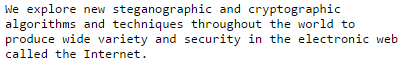
\includegraphics[scale=1]{Gambar/S0}
	\caption{Kalimat awal (S0)} 
	\label{fig:1-S0}
\end{figure}

lalu setelah disembunyikan suatu pesan dengan menggunakan \textit{line-shift coding}, muncul kalimat S1.

\begin{figure}[H]
	\centering
	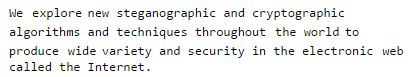
\includegraphics[scale=1]{Gambar/S1}
	\caption{Kalimat setelah melalui proses \textit{line-shift coding} (S1)} 
	\label{fig:2-S1}
\end{figure}

Dengan menumpukkan kedua kalimat S0 dan S1, didapatkan hasil sebagai berikut:

\begin{figure}[H]
	\centering
	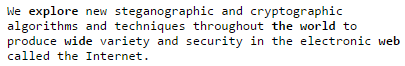
\includegraphics[scale=1]{Gambar/overlap-result}
	\caption{Hasil penumpukkan kalimat S0 dan S1} 
	\label{fig:2-overlap-result}
\end{figure}

Hasil ini dapat dicapai dengan melebarkan spasi sebelum kata \textit{explore}, \textit{the}, \textit{wide}, dan \textit{web}, juga menyempitkan spasi setelah kata \textit{explore}, \textit{world}, \textit{wide}, dan \textit{web} pada S1. Dengan demikian, kalimat yang mengandung \textit{shifted-word} akan tetap memiliki arti yang sama.

\subsubsection{Feature Coding}

\textit{Feature coding} memanfaatkan ciri yang ada dalam teks yang dapat diubah. Seperti garis lurus yang ada pada huruf b, d, h, k ,dan lain-lain. Panjang dari garis tersebut dapat diubah tanpa membuat curiga pembaca pada umumnya. Dapat juga dilakukan subtitusi pada beberapa kata dengan kata sinonimnya. Dengan itu kita dapat menyisipkan informasi 0 pada sinonim pertama dan 1 pada sinonim kedua. Cara ini harus melalui kesepakatan antara dua belah pihak tentang pasangan sinonimnya.

\subsubsection{Inter-sentence Spacing}

Cara ini akan menyandikan teks yang sudah dalam bentuk biner ke dalam teks dengan menyisipkan satu atau dua spasi setelah tiap kalimat. Misalkan satu spasi menyandikan 0 dan dua spasi menyandikan 1. Sayangnya cara ini memiliki beberapa masalah, yang pertama jika ingin menyisipkan teks yang memiliki ukuran yang besar, akan membutuhkan teks cover yang banyak pula karena 1 kalimat hanya dapat menyandikan 1 bit. Kedua, beberapa perangkat pengolah kata secara otomatis mengubah banyaknya spasi menjadi satu.

\subsubsection{End of Line Spacing}

Cara ini menyisipkan spasi pada akhir baris. Cara ini meningkatkan banyaknya informasi yang dapat disandikan dibandingkan cara sebelumnya. Sama seperti sebelumya, cara ini dapat terganggu oleh beberapa program yang dapat menghapus spasi yang berlebihan dari teks dan cara ini tidak dapat menampilkan pesan rahasia dari \textit{hard copy}.

\subsubsection{Inter-word Spacing}

Cara ketiga menggunakan spasi untuk menyandikan data yang menggunakan \textit{right-justification}. Data disandikan dengan mengatur di mana spasi ekstra akan diletakkan. Satu spasi di antara kata menyandikan 0 dan dua spasi menyandikan 1. Cara ini memungkinkan beberapa bit dapat disembunyikan dalam satu baris.

\subsection{Linguistic Steganography}
Metode ini memanfaatkan \textit{natural language processing} atau pemrosesan bahasa alami yang menyebabkan pesan dapat disembunyikan tanpa mengubah bahasa asli. Contohnya bisa dengan melakukan subtitusi terhadap sinonim yang termasuk steganografi leksikal. Perubahan dari kalimat aktif ke pasif atau sebaliknya untuk contoh dari sintaksis steganografi. Pemanfaatan suku kata untuk menyisipkan pesan yang juga termasuk ke dalam steganografi linguistik yang akan menjadi bahasan utama dalam skripsi ini.